

\documentclass{article}
\title{CSC3095:Web Platform for Digital Deployment of Virtual Servers}

\date{03.03.2017}
\author{Plamen Kolev\\ \textbf{Student number} : 130221960\\ \textbf{Supervisor} : Neil Speirs}

% USERPACKAGES
\usepackage{hyperref}

\usepackage{graphicx}
\graphicspath{ {images/} }
\usepackage{glossaries}
\usepackage{cite}
\usepackage{color}
\usepackage[english]{babel}
\usepackage{filecontents}
\usepackage[dvipsnames]{xcolor}
\usepackage[numbers,sort&compress]{natbib}
\usepackage{ifthen}
\usepackage{pgf-umlcd}
\usepackage{pdfpages}

% ENDUSERPACKAGES

% CUSTOM MACROS

\makeglossaries
\let\oldcite=\cite
\renewcommand\cite[1]{\ifthenelse{\equal{#1}{_NEEDED_}}{[citation~needed]}{\oldcite{#1}}}
% ENDCUSTOMMACROS

\definecolor{Mycolor2}{HTML}{333333}
\hypersetup{
    colorlinks,
    citecolor=blue,
    filecolor=blue,
    linkcolor=Mycolor2,
    urlcolor=blue
}

\newglossaryentry{bash}
{
	name=bash,
	description={Bourn again shell, a UNIX command line virtual shell language}
}

\newglossaryentry{open-source}{name={open-source},description={Software that makes its code openly available, allows derived work without restrictions and its distribution is done freely}}

\newglossaryentry{operating-system}
{
	name={operating system},
	description={The platform on which all user and system software is running. Examples are Windows, Linux, OSX, Android, iOSx}
}

\newglossaryentry{ssh}{
	name={ssh},
	description={
		SSH: secure shell, a network protocol that allows a remote connection to a terminal
	}
}

\begin{document}
  \pagenumbering{gobble}
  \maketitle

  \newpage
  \section{Declaration}
    I declare that this dissertation represents my own work except where otherwise stated.

  \section{Acknowledgements}


  \newpage
  \section{Abstract}

  \newpage
  \tableofcontents
  \newpage
  \listoffigures
  \newpage
  \pagenumbering{arabic}

  \newpage
  \section{Introduction}
  
    As of the year 2016, there are currently three billion people that have access to the internet \cite{ictonline}. Google handles between two and three billion search queries per day \cite{a}. Dealing with so many requests on daily basis requires full utilisation of the available hardware in terms of resources. Part of Google's ability to scale and be efficient is due to the emergence of cloud infrastructure. The topic of the paper deals  with one of the building blocks of cloud computing, which is virtualisation.
  
  \begin{quote}
  	"The quickest and cheapest method to providing the necessary level of abstraction in terms of server resource is currently virtualization..." \par\raggedleft--- \textup{Paul Robinson}, Google Cloud Computing \citeauthor{SecuringtheCloud}
  \end{quote}
  
  
  The term virtualisation is defined as the ability of one piece of hardware to run multiple operating systems \cite{b}. In this paper, a virtual machine, or an instance, is an operating system that runs on top of a "physical" operating system. The "physical" \gls{operating-system} is often referred to as the "host" system. Creating a platform that uses such technology enables an organisation to quickly set up any environment (operating system) that can be used in a variety of cases.
  
  A company that wants to buy a high performing computer for each employee would requires physical access to perform repairs and maintenance and management. Physical systems are also more difficult to manage due to their non-central distribution. Another downside is non-scalable hardware utilisation, a case where one machine uses maximum resources but another one is idle. These are some problems that virtualisation technology can deal with.  It is now a core part of most new desktop Intel© processors and is integral part of all server-grade processors.
  
  This helps with performance, as a virtual machine can be configured on the fly to use flexible amount of resources or even use shared pool of computing. This technology also allows for easy server migration, a physical machine cannot be moved within couple of minutes to a different continent. Physical infrastructure is also prone to hardware-related bugs, as a distributed software solution might not have been tested on all possible computing nodes that run it.
  
  How does virtualisation allow for easy migrations? It achieves its task by abstracting away the available physical hard drives, on the virtualisation host, they appear as a large pool of partitions with the data ready for access. Having access to the virtualisation host allows the content of such system to be copied all at once to a different provider with the only requirement that it must have enough capacity to store the information. The alternative without using a virtualisation software would be to gain physical access to each hard drive individually and copying the data incrementally.
  
  \subsection{Purpouse}
   The project aims to utilise open-source virtualisation technology and make the process of managing and creating virtual machines automated through a web interface. A system manager should be able to open a website, fill in a web form with enough information about the desired operating system, click a button and create it. 
   
   The manager should also be able to obtain and generate credentials for that machine, as well as mark common packages for installation on it. The solution should also show performance statistics and allow for network port management. These features, alongside the benefits of virtualisation should create a strong and secure infrastructure for many applications, from virtual office workstation, to server testing and deployment.
   
   Strong cryptography, virtual guest isolation, firewall rules and best practice credential and authentication methodologies and practices will be explored and will be the pillars of the system's security.
  \subsection{Aim and Objectives}
	  \subsubsection{Aim}
	  Give developers a platform for easy deployment, management and monitoring of virtual servers
	  \subsubsection{Objectives}
	  
	  \begin{enumerate}
	  	\item Deploy a virtual machine of the user's choice through shell scripts
		  	\begin{itemize}
		  		\item The main feature of the solution is the deployment of the virtual machine instances. The following will be achieved by using Oracle's virtualisation documentation for Virtualbox and the shell scripting language and the automation tool chef.
		    \end{itemize}

	  	\item Configure firewall settings
		  	\begin{itemize}
		  		\item Will be achieved through the virtualisation technology's API. Will add extra security layer to the guest operating system.
		  	\end{itemize}

	  	\item Allow console access and set up authentication credentials (SSH keys) for the instances
		  	\begin{itemize}
		  		\item The main usage of the application is to obtain a shell access to the virtual machine
		  	\end{itemize}
	  	\item Monitor disk/CPU usage of the virtual instances
	  	\item Allow the user to install software from a predefined list
	  	\item Create a website that will manage and create the machines on the behalf of the user 	
	  \end{enumerate}
  \subsection{Outline}

  \newpage
  \section{Background}
  \subsection{Similar in the field}
	For the duration of my dissertation, I have evaluated a variety of technologies, frameworks and utilities that will allow me to achieve the goal of automated system deployment. The trial and evaluation of these technologies allowed me to find the most suitable and relevant methodology for moving forward. I also experimented with different "cloud" virtual machine deployment services to understand and evaluate the key requirements that ought to be provided by the platform that I am building. 
  \subsection{Virtualisation}
  \subsection{Addoption}
  \subsection{Application}

  \newpage
  \section{Methodology}
  \subsection{Overview}
  \subsection{Planning}
  \subsection{Constrains}
  \subsection{Functional requirements}
  \subsection{Non-functional requirements}
  \subsection{Tools}

  \section{Development}
A hypervisor is a computer software or hardware that creates the platform layer to a virtual machine and makes it possible to host multiple instances with different configurations \cite{ibmvirtualisation}.

Initially, I was planning on using a hypervisor virtualisation solution such as Virtualbox and VMware, and use the \gls{bash} shell scripting language to interface directly with them. With this in mind, I decided to opt for Virtualbox, as it is an \gls{open-source} software solution, has strong community, allows third party plug-ins There are other alternatives (gnome boxes, CHROOT), but what draw me to it is that it is configurable and command-line controllable straight out of the box. Another deciding factor was also the extensibility that is offered by third party modules developed by the community.

Another reason for not choosing a more unpopular or niche technology is due to the willingness of an adopter to switch their entire virtual infrastructure to it. The Virtualbox software is very popular, and as such, it would make the transition much more subtle and unnoticeable 

As part of my research, I went through the Virtualbox command-line API. In the process of doing so, I discovered the variety of customisable parameters when building a virtual machine, like the different possibilities in setting up networks (private, network shared, host only, etc.), exposing ports, as well as different hardware configurations (RAM, hard drive, CPU count). After using the command line tools and writing a simple shell scripts for managing creation of different resources, I realised that a tool needs to be written to manage the different technical details of each virtual machine. Luckily, an open-source hypervisor provisioner software is available that helps with automation and management that satisfies the operational needs of the system. 

\subsection{Vagrant}
The tool is called Vagrant by Hashicorp, a company specialising in easy virtual machine configuration management and set-up Their API provides the following features.

	\begin{itemize}
		\item
			Allow the administrator to create a vagrant configuration file (called Vagrantfile), which describes end-to-end each operation that will be performed to the virtual machine instance (including the Linux distribution that will get installed on it).
		\item
			Create a system compatible with their platform starting from a bare configuration and incrementally building a bespoke instance. These instances can be managed and shared on the internet.
		\item
			Managing network interfaces
		\item
			Configure ports
		\item 
			Allow \gls{ssh} access
	\end{itemize}

\subsection{Architecture}
When considering the architecture of the system, a list of factors were the driving factor when building the solution. I wanted to ensure that The solution has as little moving parts as possible, which will allow it to be flexible and extensible. For that purpose I chose the programming language ruby, as it is a suitable language for system automation. Its suitability comes from the available tools vagrant and puppet which allow end-to end integration when it comes to automation. The ruby programming language also draws inspiration from the Perl programming language One of the Perl's strengths is its ability to be a more powerful shell scripting language. This is the case as it has quick syntax for executing shell scripts directly and get STDOUT, STDERR and exit-codes quickly. It does also has native implementation of common UNIX tools, like grep, wget and awk.

Because the Ruby language draws inspiration and shares similar features with Perl, it makes it a great modern and powerful language to use in this domain-specific problem.

The framework I created uses a virtual machine instance object and authenticated user that owns it. When the user fills the web form with the relevant information, it will pass the configuration values directly to a virtual machine class. This class contains a dynamic configuration, which ensures that the solution is distribution agnostic. Here, the term distribution references to the different versions of Linux (ubuntu, fedora, Centos, arch Linux). Separating dependency specific configuration by sub-classing a configuration object allows for a quick way for the project to be extended to accommodate for new distributions. 

For the purpose of this work, I have decided to limit the scope of allowed linux distributions to Ubuntu, Centos and debian, but it is important to note that the architecture allows extending that list.

To do so, folder with the name of the new distribution must be placed in lib/configurations that describes the configuration specific settings that include updating and installing common software packages.

The framework also uses UNIX environmental variable to manage infrastructure state. For the  purpose of developing and testing, I have created two main isolated environments - testing and development.
The main 

  \newpage
  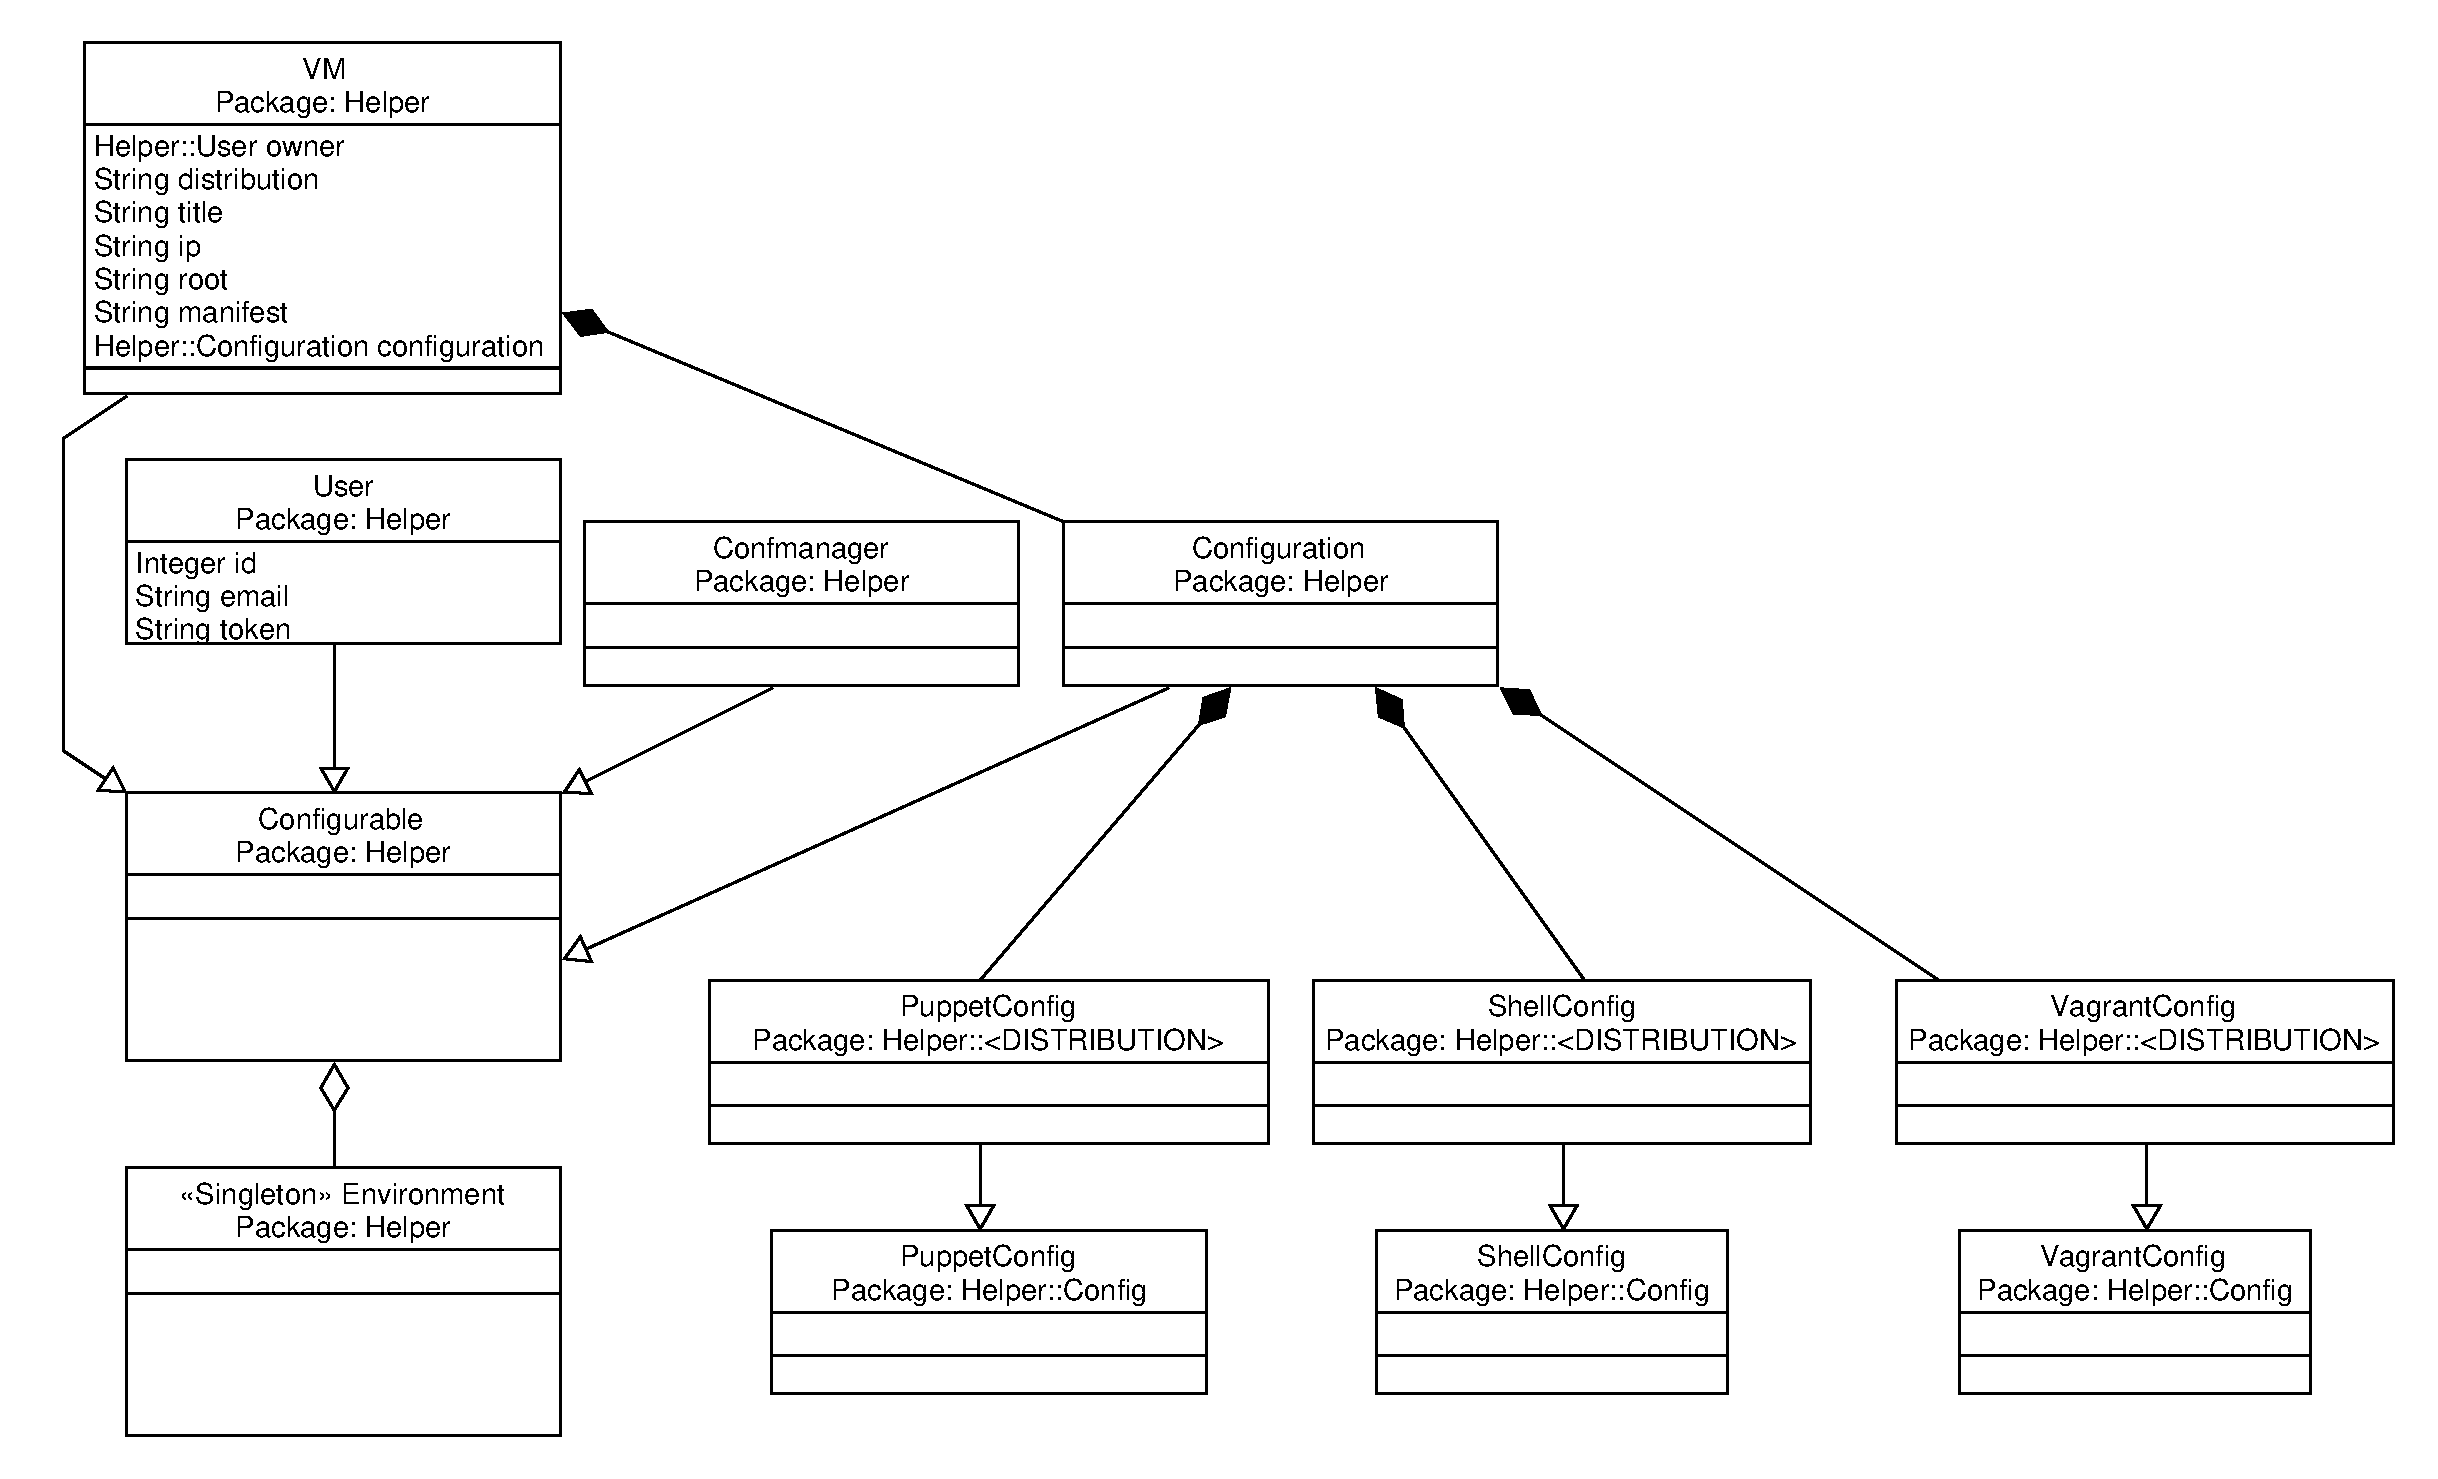
\includepdf{architecture.pdf}

  \newpage
  \section{Testing}

  \newpage
  \section{Evaluation}

  \newpage
  \section{Conclusion}

  \newpage
  \section{References}
	\bibliography{research}
	\renewcommand{\bibname}{}
  \section{Glossary}
  	\printglossary
  \newpage
  \section{Appendix}

	

	\begin{filecontents*}{research.bib}
		@online{a,
			author = {Internet Live Stats},
			title = {Google Search Statistics},
			url = {http://www.internetlivestats.com/google-search-statistics},
			urldate = {03.05.2014},
			note = {Accessed: November 26, 2016}
		},
	
		@online{b,
			author = {Techopedia Inc},
			title = {Definition of Virtualization},
			url = {https://www.techopedia.com/definition/719/virtualization},
			urldate = {2014},
			note = {Accessed: November 26, 2016}
		},
	
		@online{ictonline,
			author = {ITU ICT},
			title = {ICT Facts and Figures 2016},
			url = {http://www.itu.int/en/ITU-D/Statistics/Documents/facts/ICTFactsFigures2016.pdf},
			note = {Accessed: March 08, 2017}

		},
	
		@book{SecuringtheCloud,
			author    = {Vic (J.R.) Winkler},
			title     = {Securing the Cloud},
			year      = {2011},
			publisher = {Elsevier/Syngress},
		}
	
		@book{ibmvirtualisation,
			author    = {Shannon Meier},
			title     = {IBM Systems Virtualization: Servers, Storage, and Software},
			year      = {April 2008},
			publisher = {IBM},
		}

		
	\end{filecontents*}

	\bibliographystyle{plain}
\end{document}